% Preliminaries
\section{Preliminaries}\label{preliminaries}
	Before we define our specific data models and problems we will introduce and formalize commonly reoccurring terms.

% Graph
\subsection{Graph}
	\begin{mydef}\label{graph}
		A \textnormal{graph} $G$ is a tuple $(V, E)$ with a set of nodes $V$ and a set of
		edges $E \subseteq V \times \mathbb{R}_{\ge 0} \times V$.
		An \textnormal{edge} $e \in E$ is an ordered tuple $(u, w, v)$ with source node $u \in V$, a non-negative
		weight $w \in \mathbb{R}_{\ge 0}$ and a destination node $v \in V$.
	\end{mydef}\quad\\
	Note that \defref{graph} actually defines a \textit{directed} graph, as opposed to an \textit{undirected} graph where an
	edge like $(u, w, v)$ would be considered equal to the edge of opposite direction $(v, w, u)$ (compare to \libref{graphTheory}).
	However, for transportation networks an undirected graph often is not applicable, for example due to one way streets or
	time dependent connections like trains which depart at different times for different directions.
	
	In the context of route planning we refer to the weight $w$ of an edge $(u, w, v)$ as \textit{cost}. It can be used to encode the length
	of the represented connection. Or to represent the time it takes to travel the distance in a given
	transportation mode.
	% Graph example
	\begin{figure}[!ht]
		\begin{center}
			 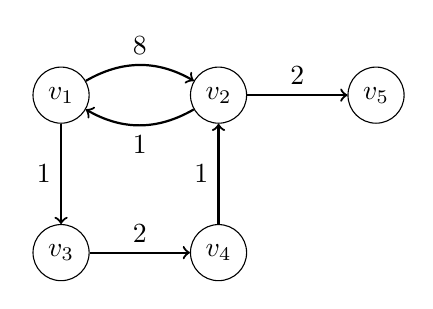
\begin{tikzpicture}[y = -1cm]
			 	% Nodes
			 	\node[circle, draw] (v1) at (0, 0) {$v_1$};
			 	\node[circle, draw] (v2) at (2, 0) {$v_2$};
			 	\node[circle, draw] (v3) at (0, 2) {$v_3$};
			 	\node[circle, draw] (v4) at (2, 2) {$v_4$};
			 	\node[circle, draw] (v5) at (4, 0) {$v_5$};
			 	
			 	% Edges
			 	\draw[thick, ->] (v1) to [bend left] node[above] {$8$} (v2);
			 	\draw[thick, ->] (v2) to node[above] {$2$} (v5);
			 	\draw[thick, ->] (v2) to [bend left] node[below] {$1$} (v1);
			 	\draw[thick, ->] (v1) to node[left] {$1$} (v3);
			 	\draw[thick, ->] (v3) to node[above] {$2$} (v4);
			 	\draw[thick, ->] (v4) to node[left] {$1$} (v2);
			\end{tikzpicture}
		\end{center}
		\caption{Illustration of an example graph with five nodes and six edges.}
		\label{graph_example}
	\end{figure}\quad\\
	As an example consider the graph $G = (V, E)$ with
	\begin{align*}
		V	&= \{v_1, v_2, v_3, v_4, v_5\} \text{ and}\\
		E	&= \{(v_1, 8, v_2), (v_1, 1, v_3), (v_2, 1, v_1), (v_2, 2, v_5), (v_3, 2, v_4), (v_4, 1, v_2)\}.
	\end{align*}
	which is illustrated by \figref{graph_example}.
	\begin{mydef}
		Given a graph $G = (V, E)$ the function $\src: E \to V, ((u, w, v)) \mapsto u$ gets the \textnormal{source}
		of an edge. Analogously $\dest: E \to V, ((u, w, v)) \mapsto v$ retrieves the \textnormal{destination}.
	\end{mydef}
	\begin{mydef}\label{path}
		A \textnormal{path} in a graph $G = (V, E)$ is a sequence $p = e_1e_2e_3\ldots$ of edges $e_i \in E$ such that
		\begin{align*}
			\forall i: \dest(e_i) = \src(e_{i + 1}).
		\end{align*}
		The \textnormal{length} of a path is the amount of edges it contains, i.e. the length of the sequence.
		The \textnormal{weight} or \textnormal{cost} is the sum of its edges weights.
	\end{mydef}\quad\\
	An example for a path in the graph $G$ would be
	\begin{align*}
		p	&=(v_1, 8, v_2)(v_2, 1, v_1)(v_1, 1, v_3).
	\end{align*}
	Its length is $3$ and it has a weight of $10$.
	
% Tree
\subsection{Tree}
	\begin{mydef}\label{tree}
		A \textnormal{tree} is a graph $T = (V, E)$ with the following properties:
		\begin{itemize}
			\item[1.] There is exactly one node $r \in V$ with no ingoing edges, called the \textnormal{root}, i.e.
				\begin{align*}
					\exists! r \in V \nexists e \in E : \dest(e) = r.
				\end{align*}
			\item[2.] All other nodes $v$ have exactly one ingoing edge. The source $p$ of this edge is called \textnormal{parent} of $v$ and
				$v$ is called \textnormal{child} of $p$:
				\begin{align*}
					\forall v \in V : v \neq r \Rightarrow \exists! e \in E : \dest(e) = v.
				\end{align*}
		\end{itemize}
	\end{mydef}
	\begin{mydef}\label{subTree}
		The \textnormal{subtree} of a tree $T = (V, E)$ rooted at a node $r' \in V$ is a tree $T' = (V', E')$. $V' \subseteq V$ is the set
		of nodes that can be reached from $r'$. That is, all nodes that are part of possible paths starting at $r'$.
		Likewise $E' \subseteq E$ is the set of edges restricted to the vertices in $V'$. The root of $T'$ is $r'$.
	\end{mydef}
	\begin{mydef}\label{treeDepth}
		The \textnormal{depth} of a node $v$ in a tree $T = (V, E)$, denoted by $\depth(v)$, is defined as the amount of
		edges between the $v$ and the root $r$. It is the length of the unique path $p$ starting at $r$ and ending at $v$.
		
		The \textnormal{height} of a tree is its greatest depth, i.e.
		\begin{align*}
			\max_{v \in V} \depth(v).
		\end{align*}
		And
		\begin{align*}
			\children(v)	&= \{c \in T | c \text{ child of } v\}.
		\end{align*}
	\end{mydef}\quad\\
	Trees are hierarchical data structures. Every node, except the root, has one parent. A node itself can have multiple children.
	Note that it is not possible to form a loop in a tree, i.e. a path that visits a node more than once. A node without
	children is called a \textit{leaf}.\todo{Maybe add some illustrations here...}

% Metric
\subsection{Metric}
	\begin{mydef}\label{metric}
		A function $d: M \times M \to \mathbb{R}$ on a set $M$ is called a \textnormal{metric} iff for all $x, y, z \in M$
		\begin{align*}
			d(x, y)	&\ge 0,			&&\text{non-negativity}\\
			d(x, y) = 0	&\Leftrightarrow x = y,	&&\text{identity of indiscernibles}\\
			d(x, y)	&= d(y, x) \text{ and }	&&\text{symmetry}\\
			d(x, z)	&\le d(x, y) + d(y, z)	&&\text{triangle inequality}
		\end{align*}
		holds.
	\end{mydef}
	\begin{mydef}\label{metricSpace}
		A \textnormal{metric space} is a pair $(M, d)$ where $M$ is a set
		and $d: M \times M \to \mathbb{R}$ a metric on $M$.
	\end{mydef}
	\begin{mydef}\label{metricSet}
		Given a metric $d$ on a set $M$, the distance of a point $p \in M$ to a subset $Q \subseteq M$
		is defined as the distance from $p$ to its nearest point in $Q$:
		\begin{align*}
			d(p, Q)	&= \min_{q \in Q} d(p, q)
		\end{align*}
	\end{mydef}\quad\\
	A metric is used to measure the distance between given locations. \sectionref{nearestNeighborProblem}
	and \sectionref{shortestPathProblem}, in particular \sectionref{alt}, will make heavy use of this term.
	
	There we measure the distance between geographical locations given as pair of \textit{latitude} and \textit{longitude} coordinates.
	Latitude and longitude, often denoted by $\phi$ and $\lambda$, are real numbers in the ranges $(-90, 90)$ and $[-180, 180)$ respectively,
	measured in degrees. However, for convenience we represent them in radians. Both representations are equivalent to each other
	and can easily be converted using the ratio $360^\circ = 2 \pi \text{ rad}$.\\\\
	A commonly used measure is the \textit{as-the-crow-flies} metric, which is equivalent to the euclidean distance in the euclidean space.
	\defref{asTheCrowFlies} defines an approximation of this distance on locations given by latitude and longitude coordinates.
	The approximation is commonly known as equirectangular projection of the earth \libref{equiRectProjection}.
	Note that there are more accurate methods for computing the great-circle distance for geographical locations,
	like the haversine formula \libref{haversine}. However, they come with a significant computational overhead.
	\begin{mydef}\label{asTheCrowFlies}
		Given a set of coordinates $M = \left\{(\phi, \lambda) | \phi \in \left(-\frac{\pi}{2}, \frac{\pi}{2}\right), \lambda \in [-\pi, \pi)\right\}$ we define
		$\asTheCrowFlies: M \times M \to \mathbb{R}$ such that
		\begin{align*}
			\left(\left(\phi_1, \lambda_1\right), \left(\phi_2, \lambda_2\right)\right) \mapsto
				\sqrt{\left(\left(\lambda_2 - \lambda_1\right) \cdot \cos\left(\frac{\phi_1 + \phi_2}{2}\right)\right)^2
					+ \left(\phi_2 - \phi_1\right)^2} \cdot 6371000.
		\end{align*}
	\end{mydef}\quad\\
	As a next step we prove that $\asTheCrowFlies$ is indeed a metric on the set of coordinates.
	\begin{myproposition}
		The function $\asTheCrowFlies$ is a metric on its domain $M$.
	\end{myproposition}
	\begin{proof}
		We need to prove that all four axioms hold. Let us first set
		\begin{align*}
			x	&= \left(\lambda_2 - \lambda_1\right) \cdot \cos\left(\frac{\phi_1 + \phi_2}{2}\right)\\
			y	&= \phi_2 - \phi_1
		\end{align*}
		then the function simplifies to
		\begin{align*}
			\sqrt{x^2 + y^2} \cdot 6371000.
		\end{align*}
		Obviously this can never resolve to a negative number since
		\begin{align*}
			\underbrace{\underbrace{\sqrt{\underbrace{x^2}_{\ge 0} + \underbrace{y^2}_{\ge 0}}}_{\ge 0} \cdot 6371000}_{\ge 0}.
		\end{align*}
		
		For the second axiom we assume that $\asTheCrowFlies\left(\left(\phi_1, \lambda_1\right), \left(\phi_2, \lambda_2\right)\right) = 0$
		for an arbitrary pair of coordinates and follow\\
		\begin{center}
			\begin{tabular}{RRL}
							&\sqrt{\left(\left(\lambda_2 - \lambda_1\right) \cdot \cos\left(\frac{\phi_1 + \phi_2}{2}\right)\right)^2
								+ \left(\phi_2 - \phi_1\right)^2} \cdot 6371000	&= 0\\
				\Leftrightarrow	&\sqrt{\left(\left(\lambda_2 - \lambda_1\right) \cdot \cos\left(\frac{\phi_1 + \phi_2}{2}\right)\right)^2
								+ \left(\phi_2 - \phi_1\right)^2} 				&= 0\\
				\Leftrightarrow	&\left(\left(\lambda_2 - \lambda_1\right) \cdot \cos\left(\frac{\phi_1 + \phi_2}{2}\right)\right)^2
								+ \left(\phi_2 - \phi_1\right)^2 				&= 0
			\end{tabular}
		\end{center}
		At this point either both summands are $0$ or one is the negative of the other. However, both summands must be positive due to the quadration.
		Because of that we follow\\
		\begin{center}
			\begin{tabular}{RRL}
							&\left(\phi_2 - \phi_1\right)^2 	&= 0\\
				\Leftrightarrow	&\phi_2				&= \phi_1
			\end{tabular}
		\end{center}
		and with that\\
		\begin{center}
			\begin{tabular}{RRL}
							&\left(\left(\lambda_2 - \lambda_1\right) \cdot \cos\left(\frac{\phi_1 + \phi_2}{2}\right)\right)^2	&= 0\\
				\Leftrightarrow	&\left(\lambda_2 - \lambda_1\right) \cdot \cos\left(\frac{2 \phi_1}{2}\right)	&= 0\\
				\Leftrightarrow	&\left(\lambda_2 - \lambda_1\right) \cdot \cos\left(\phi_1\right)	&= 0.
			\end{tabular}
		\end{center}
		Since $\phi_1 \in \left(-\frac{\pi}{2}, \frac{\pi}{2}\right)$ it follows that $\cos\left(\phi_1\right) \ne 0$. As such
		\begin{center}
			\begin{tabular}{RRL}
							&\lambda_2 - \lambda_1	&= 0\\
				\Leftrightarrow	&\lambda_2			&= \lambda_1
			\end{tabular}
		\end{center}
		and by that $(\phi_1, \lambda_1) = (\phi_2, \lambda_2)$, so the second axiom holds.
		
		Symmetry follows quickly since
		\begin{align*}
			\phi_1 + \phi_2	&= \phi_2 + \phi_1\\
			(\phi_2 - \phi_1)^2	&= (\phi_1 - \phi_2)^2\\
			\left((\lambda_2 - \lambda_1) \cdot \cos\left(\frac{\phi_1 + \phi_2}{2}\right)\right)^2
				&= (\lambda_2 - \lambda_1)^2 \cdot \cos^2\left(\frac{\phi_1 + \phi_2}{2}\right)\\
			(\lambda_2 - \lambda_1)^2	&= (\lambda_1 - \lambda_2)^2.
		\end{align*}
		
		The triangle inequality is a bit trickier, we choose three arbitrary coordinates $c_i = (\phi_i, \lambda_i)$ for $i = 1, 2, 3$
		and start on the squared left side:
		\begin{align*}
			\asTheCrowFlies^2(c_1, c_3)
				&= \left(\left(\left(\lambda_3 - \lambda_1\right) \cdot \cos\left(\frac{\phi_1 + \phi_3}{2}\right)\right)^2
					+ \left(\phi_3 - \phi_1\right)^2\right) \cdot 6371000^2\\
				&= \left(\left(\left(\lambda_3 - \lambda_2 + \lambda_2 - \lambda_1\right) \cdot \cos\left(\frac{\phi_1 + \phi_3}{2}\right)\right)^2
					+ \left(\phi_3 - \phi_2 + \phi_2 - \phi_1\right)^2\right) \cdot 6371000^2\\
				&= \Bigg(\left((\lambda_3 - \lambda_2)^2 + (\lambda_2 - \lambda_1)^2 + 2 \cdot ((\lambda_3 - \lambda_2) \cdot (\lambda_2 - \lambda_1))\right)
						\cdot \cos^2\left(\frac{\phi_1 + \phi_3}{2}\right)\\
					&\qquad + (\phi_3 - \phi_2)^2 + (\phi_2 - \phi_1)^2 + 2 \cdot ((\pi_3 - \phi_2) \cdot (\phi_2 - \phi_1))\Bigg) \cdot 6371000^2\\
				&= ...\\
				&\le \left(\left(\left(\left(\lambda_2 - \lambda_1\right) \cdot \cos\left(\frac{\phi_1 + \phi_2}{2}\right)\right)^2
						+ \left(\phi_2 - \phi_1\right)^2\right) \cdot 6371000^2\right)\\
					&\qquad+ \left(\left(\left(\left(\lambda_3 - \lambda_2\right) \cdot \cos\left(\frac{\phi_2 + \phi_3}{2}\right)\right)^2
						+ \left(\phi_3 - \phi_2\right)^2\right) \cdot 6371000^2\right)\\
					&\qquad + 2 \cdot \left(\left(\left(\left(\lambda_2 - \lambda_1\right) \cdot \cos\left(\frac{\phi_1 + \phi_2}{2}\right)\right)^2
						+ \left(\phi_2 - \phi_1\right)^2\right) \cdot 6371000^2\right)\\
					&\qquad \cdot \left(\left(\left(\left(\lambda_3 - \lambda_2\right) \cdot \cos\left(\frac{\phi_2 + \phi_3}{2}\right)\right)^2
						+ \left(\phi_3 - \phi_2\right)^2\right) \cdot 6371000^2\right)\\
				&= \left(\asTheCrowFlies(c_1, c_2) + \asTheCrowFlies(c_2, c_3)\right)^2
		\end{align*}
		\todo{continue (squared ineq holds without, cauchy schwarz ineq) or remove completely...}
		All four axioms hold, $\asTheCrowFlies$ is a metric on the set $M$.
	\end{proof}